\documentclass{standalone}
\usepackage{tikz}
\usetikzlibrary{positioning}

\tikzset{
	grainenv/.pic = {
	 \coordinate (-center) at (0,0) ;
	 \coordinate (-right) at (3,.5) ;
	 \coordinate (-left) at (0,.5) ;
     \draw [domain=0:3, samples=200] plot (\x, {sin(60*\x)});
     \draw [thin] (0,0) rectangle (3,1);
     \node [anchor=center] at (1.5,1.2) {Grain envelope};
     \node [anchor=center] at (-0.1,0) {\tiny 0};
     \node [anchor=center] at (-0.1,1) {\tiny 1};
     }}

\tikzset{
	grainwav/.pic = {
	 \coordinate (-right) at (3,.5) ;
     \draw [domain=0:3, samples=200] plot (\x, {sin(120*\x)/2+1/2});
     \draw [thin] (0,0) rectangle (3,1);
     \draw [thin] (0,.5) -- (3,.5);
     \node [anchor=center] at (1.5,1.2) {Grain waveform};
     \node [anchor=center] at (-0.1,0) {\tiny -1};
     \node [anchor=center] at (-.1,.5) {\tiny 0};
     \node [anchor=center] at (-0.1,1) {\tiny 1};
     }}

\tikzset{
	osc/.pic = {
	 \coordinate (-inleft) at (-0.8,0) ;
	 \coordinate (-inright) at (0.8,0) ;
	 \coordinate (-out) at (0,-1.5) ;
	 \coordinate (-center) at (0,-0.7) ;
	 \coordinate (-right) at (1.3,-.7) ;
	 \coordinate (-left) at (-1.3,-.7) ;
	 \draw (-1.5,0) -- (1.5,0) arc (0:-180:1.5) --cycle;
	 }
	}
	

\begin{document} \sffamily
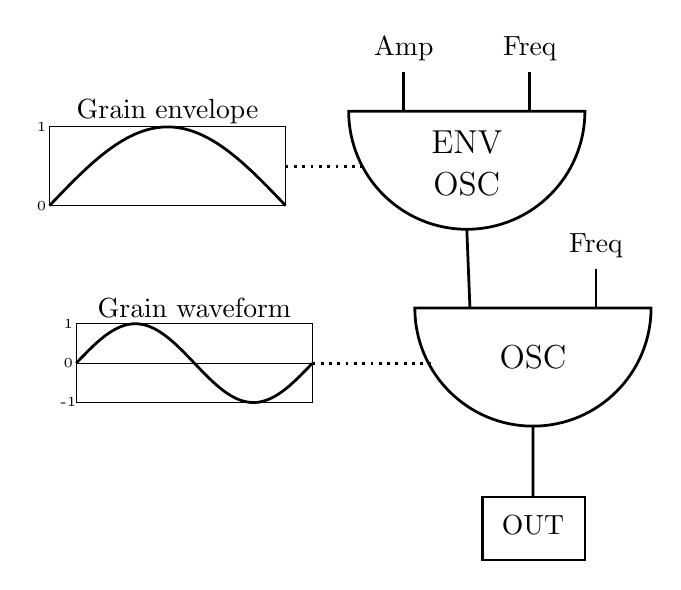
\begin{tikzpicture}[node distance=1, line width=1pt]

% NODES

% env osc
\pic (envosc) {osc};
\node (envosclabel) [above=of envosc-out,yshift=-.7cm,align=center] {\large ENV \\[.1cm] \large OSC};
\node (envoscamp) [above=of envosc-inleft,yshift=-.5cm] {Amp};
\node (envoscfreq) [above=of envosc-inright,yshift=-.5cm] {Freq};
\pic (grenv) [left=of envosc-left, xshift=-3cm, yshift=-.5cm] {grainenv};

% wave osc, out
\pic (wavosc) [below=of envosc-out,xshift=.84cm] {osc};
\node (wavosclabel) [above=of wavosc-out,yshift=-.4cm,align=center] {\large OSC};
\node (wavoscfreq) [above=of wavosc-inright,yshift=-.5cm] {Freq};
\pic (grainwav) [left=of wavosc-left, xshift=-3.5cm,yshift=-.5cm] {grainwav};
\draw (0.2,-5.7) rectangle (1.5,-4.9);
\node (out) [below=of wavosc-out] {OUT};


%CONNECTIONS
\draw (envoscamp) -- (envosc-inleft);
\draw (envoscfreq) -- (envosc-inright);
\draw (envosc-out) -- (wavosc-inleft);
\draw (wavoscfreq) -- (wavosc-inright);
\draw (wavosc-out) -- (0.84,-4.9);
\draw [dotted] (grenv-right) -- (envosc-left);
\draw [dotted] (grainwav-right) -- (wavosc-left);

\end{tikzpicture}
\end{document}